\chapter{プログラムで、いろいろ自動化してみよう}
\section{条件判断の使い方}

今回もまず、プログラミングのツールHSP(Hot SoupProcessor)を起動して、
スクリプトを実行するための準備を始めましょう。
左上のRaspberry Piメニューの「プログラミング」項目にある、
「HSP Script Editor」(HSPスクリプトエディタ)からエディタを起動してください。

\begin{figure}[H]
  \begin{center}
    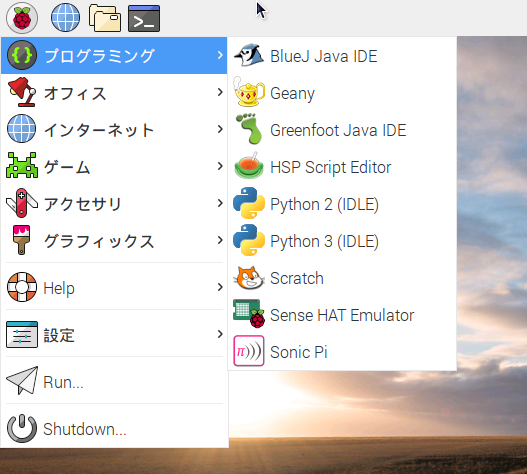
\includegraphics[width=6.489cm,height=5.826cm]{images/chap04/text04-img001.png}
    \caption{プログラミング項目のメニュー}
  \end{center}
  %\label{fig:prog_menu}
\end{figure}

まずは、教材のスクリプトを動かして試してみましょう。
ファイル→「開く」メニューから/home/pi/ome/04ディレクトリの中にある
「swhandan.hsp」を読み込んでください。
作業は、すべて「pi」から選択できる「ome/04」ディレクトリで行います。
見つからない場合は、まわりの友達か、近くの先生に聞いてみてください。

\begin{figure}[H]
  \begin{center}
    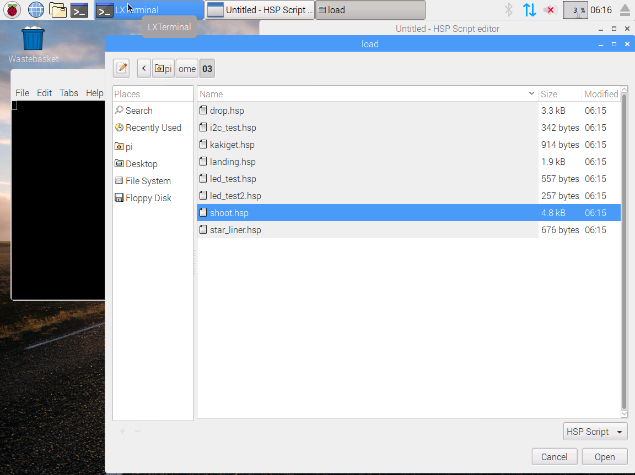
\includegraphics[width=7.338cm,height=5.493cm]{images/chap04/text04-img002.png}
    \caption{ディレクトリから読み込む画面}
  \end{center}
  \label{fig:read_from_directory}
\end{figure}

\clearpage

